% Options for packages loaded elsewhere
\PassOptionsToPackage{unicode}{hyperref}
\PassOptionsToPackage{hyphens}{url}
%
\documentclass[
  ignorenonframetext,
]{beamer}
\usepackage{pgfpages}
\setbeamertemplate{caption}[numbered]
\setbeamertemplate{caption label separator}{: }
\setbeamercolor{caption name}{fg=normal text.fg}
\beamertemplatenavigationsymbolsempty
% Prevent slide breaks in the middle of a paragraph
\widowpenalties 1 10000
\raggedbottom
\setbeamertemplate{part page}{
  \centering
  \begin{beamercolorbox}[sep=16pt,center]{part title}
    \usebeamerfont{part title}\insertpart\par
  \end{beamercolorbox}
}
\setbeamertemplate{section page}{
  \centering
  \begin{beamercolorbox}[sep=12pt,center]{part title}
    \usebeamerfont{section title}\insertsection\par
  \end{beamercolorbox}
}
\setbeamertemplate{subsection page}{
  \centering
  \begin{beamercolorbox}[sep=8pt,center]{part title}
    \usebeamerfont{subsection title}\insertsubsection\par
  \end{beamercolorbox}
}
\AtBeginPart{
  \frame{\partpage}
}
\AtBeginSection{
  \ifbibliography
  \else
    \frame{\sectionpage}
  \fi
}
\AtBeginSubsection{
  \frame{\subsectionpage}
}

\usepackage{amsmath,amssymb}
\usepackage{iftex}
\ifPDFTeX
  \usepackage[T1]{fontenc}
  \usepackage[utf8]{inputenc}
  \usepackage{textcomp} % provide euro and other symbols
\else % if luatex or xetex
  \usepackage{unicode-math}
  \defaultfontfeatures{Scale=MatchLowercase}
  \defaultfontfeatures[\rmfamily]{Ligatures=TeX,Scale=1}
\fi
\usepackage{lmodern}
\usetheme[]{Boadilla}
\usecolortheme{rose}
\ifPDFTeX\else  
    % xetex/luatex font selection
\fi
% Use upquote if available, for straight quotes in verbatim environments
\IfFileExists{upquote.sty}{\usepackage{upquote}}{}
\IfFileExists{microtype.sty}{% use microtype if available
  \usepackage[]{microtype}
  \UseMicrotypeSet[protrusion]{basicmath} % disable protrusion for tt fonts
}{}
\makeatletter
\@ifundefined{KOMAClassName}{% if non-KOMA class
  \IfFileExists{parskip.sty}{%
    \usepackage{parskip}
  }{% else
    \setlength{\parindent}{0pt}
    \setlength{\parskip}{6pt plus 2pt minus 1pt}}
}{% if KOMA class
  \KOMAoptions{parskip=half}}
\makeatother
\usepackage{xcolor}
\newif\ifbibliography
\setlength{\emergencystretch}{3em} % prevent overfull lines
\setcounter{secnumdepth}{-\maxdimen} % remove section numbering

\usepackage{color}
\usepackage{fancyvrb}
\newcommand{\VerbBar}{|}
\newcommand{\VERB}{\Verb[commandchars=\\\{\}]}
\DefineVerbatimEnvironment{Highlighting}{Verbatim}{commandchars=\\\{\}}
% Add ',fontsize=\small' for more characters per line
\usepackage{framed}
\definecolor{shadecolor}{RGB}{241,243,245}
\newenvironment{Shaded}{\begin{snugshade}}{\end{snugshade}}
\newcommand{\AlertTok}[1]{\textcolor[rgb]{0.68,0.00,0.00}{#1}}
\newcommand{\AnnotationTok}[1]{\textcolor[rgb]{0.37,0.37,0.37}{#1}}
\newcommand{\AttributeTok}[1]{\textcolor[rgb]{0.40,0.45,0.13}{#1}}
\newcommand{\BaseNTok}[1]{\textcolor[rgb]{0.68,0.00,0.00}{#1}}
\newcommand{\BuiltInTok}[1]{\textcolor[rgb]{0.00,0.23,0.31}{#1}}
\newcommand{\CharTok}[1]{\textcolor[rgb]{0.13,0.47,0.30}{#1}}
\newcommand{\CommentTok}[1]{\textcolor[rgb]{0.37,0.37,0.37}{#1}}
\newcommand{\CommentVarTok}[1]{\textcolor[rgb]{0.37,0.37,0.37}{\textit{#1}}}
\newcommand{\ConstantTok}[1]{\textcolor[rgb]{0.56,0.35,0.01}{#1}}
\newcommand{\ControlFlowTok}[1]{\textcolor[rgb]{0.00,0.23,0.31}{#1}}
\newcommand{\DataTypeTok}[1]{\textcolor[rgb]{0.68,0.00,0.00}{#1}}
\newcommand{\DecValTok}[1]{\textcolor[rgb]{0.68,0.00,0.00}{#1}}
\newcommand{\DocumentationTok}[1]{\textcolor[rgb]{0.37,0.37,0.37}{\textit{#1}}}
\newcommand{\ErrorTok}[1]{\textcolor[rgb]{0.68,0.00,0.00}{#1}}
\newcommand{\ExtensionTok}[1]{\textcolor[rgb]{0.00,0.23,0.31}{#1}}
\newcommand{\FloatTok}[1]{\textcolor[rgb]{0.68,0.00,0.00}{#1}}
\newcommand{\FunctionTok}[1]{\textcolor[rgb]{0.28,0.35,0.67}{#1}}
\newcommand{\ImportTok}[1]{\textcolor[rgb]{0.00,0.46,0.62}{#1}}
\newcommand{\InformationTok}[1]{\textcolor[rgb]{0.37,0.37,0.37}{#1}}
\newcommand{\KeywordTok}[1]{\textcolor[rgb]{0.00,0.23,0.31}{#1}}
\newcommand{\NormalTok}[1]{\textcolor[rgb]{0.00,0.23,0.31}{#1}}
\newcommand{\OperatorTok}[1]{\textcolor[rgb]{0.37,0.37,0.37}{#1}}
\newcommand{\OtherTok}[1]{\textcolor[rgb]{0.00,0.23,0.31}{#1}}
\newcommand{\PreprocessorTok}[1]{\textcolor[rgb]{0.68,0.00,0.00}{#1}}
\newcommand{\RegionMarkerTok}[1]{\textcolor[rgb]{0.00,0.23,0.31}{#1}}
\newcommand{\SpecialCharTok}[1]{\textcolor[rgb]{0.37,0.37,0.37}{#1}}
\newcommand{\SpecialStringTok}[1]{\textcolor[rgb]{0.13,0.47,0.30}{#1}}
\newcommand{\StringTok}[1]{\textcolor[rgb]{0.13,0.47,0.30}{#1}}
\newcommand{\VariableTok}[1]{\textcolor[rgb]{0.07,0.07,0.07}{#1}}
\newcommand{\VerbatimStringTok}[1]{\textcolor[rgb]{0.13,0.47,0.30}{#1}}
\newcommand{\WarningTok}[1]{\textcolor[rgb]{0.37,0.37,0.37}{\textit{#1}}}

\providecommand{\tightlist}{%
  \setlength{\itemsep}{0pt}\setlength{\parskip}{0pt}}\usepackage{longtable,booktabs,array}
\usepackage{calc} % for calculating minipage widths
\usepackage{caption}
% Make caption package work with longtable
\makeatletter
\def\fnum@table{\tablename~\thetable}
\makeatother
\usepackage{graphicx}
\makeatletter
\def\maxwidth{\ifdim\Gin@nat@width>\linewidth\linewidth\else\Gin@nat@width\fi}
\def\maxheight{\ifdim\Gin@nat@height>\textheight\textheight\else\Gin@nat@height\fi}
\makeatother
% Scale images if necessary, so that they will not overflow the page
% margins by default, and it is still possible to overwrite the defaults
% using explicit options in \includegraphics[width, height, ...]{}
\setkeys{Gin}{width=\maxwidth,height=\maxheight,keepaspectratio}
% Set default figure placement to htbp
\makeatletter
\def\fps@figure{htbp}
\makeatother

\makeatletter
\makeatother
\makeatletter
\makeatother
\makeatletter
\@ifpackageloaded{caption}{}{\usepackage{caption}}
\AtBeginDocument{%
\ifdefined\contentsname
  \renewcommand*\contentsname{Table of contents}
\else
  \newcommand\contentsname{Table of contents}
\fi
\ifdefined\listfigurename
  \renewcommand*\listfigurename{List of Figures}
\else
  \newcommand\listfigurename{List of Figures}
\fi
\ifdefined\listtablename
  \renewcommand*\listtablename{List of Tables}
\else
  \newcommand\listtablename{List of Tables}
\fi
\ifdefined\figurename
  \renewcommand*\figurename{Figure}
\else
  \newcommand\figurename{Figure}
\fi
\ifdefined\tablename
  \renewcommand*\tablename{Table}
\else
  \newcommand\tablename{Table}
\fi
}
\@ifpackageloaded{float}{}{\usepackage{float}}
\floatstyle{ruled}
\@ifundefined{c@chapter}{\newfloat{codelisting}{h}{lop}}{\newfloat{codelisting}{h}{lop}[chapter]}
\floatname{codelisting}{Listing}
\newcommand*\listoflistings{\listof{codelisting}{List of Listings}}
\makeatother
\makeatletter
\@ifpackageloaded{caption}{}{\usepackage{caption}}
\@ifpackageloaded{subcaption}{}{\usepackage{subcaption}}
\makeatother
\makeatletter
\@ifpackageloaded{tcolorbox}{}{\usepackage[skins,breakable]{tcolorbox}}
\makeatother
\makeatletter
\@ifundefined{shadecolor}{\definecolor{shadecolor}{rgb}{.97, .97, .97}}
\makeatother
\makeatletter
\makeatother
\makeatletter
\makeatother
\ifLuaTeX
  \usepackage{selnolig}  % disable illegal ligatures
\fi
\IfFileExists{bookmark.sty}{\usepackage{bookmark}}{\usepackage{hyperref}}
\IfFileExists{xurl.sty}{\usepackage{xurl}}{} % add URL line breaks if available
\urlstyle{same} % disable monospaced font for URLs
\hypersetup{
  pdftitle={Array-Based Data Structures, Searching, and Sorting},
  pdfauthor={Salaar Liaqat},
  hidelinks,
  pdfcreator={LaTeX via pandoc}}

\title{Array-Based Data Structures, Searching, and Sorting}
\author{Salaar Liaqat}
\date{}
\institute{Data Sciences Institute, UofT}

\begin{document}
\frame{\titlepage}
\ifdefined\Shaded\renewenvironment{Shaded}{\begin{tcolorbox}[interior hidden, borderline west={3pt}{0pt}{shadecolor}, frame hidden, boxrule=0pt, breakable, sharp corners, enhanced]}{\end{tcolorbox}}\fi

\begin{frame}{Outline}
\protect\hypertarget{outline}{}
\begin{itemize}
\item
  Array Based Data Structures

  \begin{itemize}
  \tightlist
  \item
    Stack, queue, Python List
  \end{itemize}
\item
  Searching

  \begin{itemize}
  \tightlist
  \item
    Linear, Binary Search
  \end{itemize}
\item
  Sorting

  \begin{itemize}
  \tightlist
  \item
    Selection, Insertion Sort
  \end{itemize}
\item
  Hash map, hash table (Python dictionary), hash functions
\end{itemize}
\end{frame}

\hypertarget{array-based-data-structures}{%
\section{Array Based Data
Structures}\label{array-based-data-structures}}

\begin{frame}{Abstract Data Types Versus Data Structure}
\protect\hypertarget{abstract-data-types-versus-data-structure}{}
\begin{itemize}
\item
  Some concepts are generally useful and transcend any programming
  language
\item
  An \textbf{abstract data type} (ADT) defines some kind of data and
  operations that can be performed on it

  \begin{itemize}
  \item
    Abstract because there is no mention of \emph{how} data is stored or
    \emph{how} the operations work
  \item
    Concerned about ``what''
  \end{itemize}
\item
  A \textbf{data structure} is a concrete method of storing data (and
  therefore its operations).

  \begin{itemize}
  \tightlist
  \item
    For instance, Python List is a data structure because it has a
    specific implementation.
  \end{itemize}
\item
  ADTs form a common vocabulary for computer scientists to discuss
  problems. It allows us to focus on the design and worry about
  implementation later.
\end{itemize}
\end{frame}

\begin{frame}{Important ADTs}
\protect\hypertarget{important-adts}{}
\begin{itemize}
\item
  Set

  \begin{itemize}
  \item
    Data: a collection of unique elements
  \item
    Operations: get size, insert a value (without introducing
    duplicates), remove a specified value, check membership
  \end{itemize}
\item
  List

  \begin{itemize}
  \item
    Data: an ordered sequence of elements
  \item
    Operations: access element by index, insert a value at a given
    index, remove a value at a given index
  \end{itemize}
\end{itemize}
\end{frame}

\begin{frame}{Important ADTs \footnote<.->{From
  https://www.teach.cs.toronto.edu/\textasciitilde csc148h/winter/notes/}}
\protect\hypertarget{important-adts-1}{}
\begin{itemize}
\item
  Map

  \begin{itemize}
  \item
    Data: a collection of key-value pairs, where each key is unique and
    associated with a single value
  \item
    Operations: look-up a value for a given key, insert a new key-value
    pair, remove a key-value pair, update the value associated with a
    given key
  \end{itemize}
\item
  Iterable

  \begin{itemize}
  \item
    Data: a collection of values (may or may not be unique)
  \item
    Operations: iterate through the elements of the collection one at a
    time.
  \end{itemize}
\end{itemize}
\end{frame}

\begin{frame}[fragile]{Relation between ADTs and Data Structures}
\protect\hypertarget{relation-between-adts-and-data-structures}{}
\begin{itemize}
\item
  A Python \texttt{list} is not a ADT. But it is a natural
  implementation of the List ADT.

  \begin{itemize}
  \tightlist
  \item
    The designers of Python implemented \texttt{list} operations
  \end{itemize}
\item
  A single ADT can be implemented by many data structures

  \begin{itemize}
  \item
    You could implement List ADT using a Python \texttt{dict}
  \item
    We can store the list \texttt{{[}"DS",\ 4,\ "Life"{]}} like this:
    \texttt{\{0:\ "DS",\ 1:\ 4,\ 2:\ "Life"\}}
  \end{itemize}
\item
  A data structure can implement many ADTs

  \begin{itemize}
  \tightlist
  \item
    Practice: how can you implement a set with a Python \texttt{list}?
  \end{itemize}
\end{itemize}
\end{frame}

\begin{frame}[fragile]{Python Lists}
\protect\hypertarget{python-lists}{}
\begin{itemize}
\item
  Each element has an address in memory. The addresses are ordered by
  index number and adjacent to each other.
\item
  Run time for \texttt{append} method

  \begin{itemize}
  \item
    A new address is created and placed at the end of the list
  \item
    \(O(1)\) time because it doesn't matter how long the list is
  \end{itemize}
\item
  Run time for \texttt{insert} method

  \begin{itemize}
  \item
    The worst case occurs when you insert at the beginning of the list
    because each element in the list has to be shifted down by 1.
  \item
    \(O(n)\) time
  \end{itemize}
\item
  Run time for \texttt{delete} method

  \begin{itemize}
  \item
    If you remove the first element, all other elements must be shifted
    up by one.
  \item
    \(O(n)\) time
  \end{itemize}
\end{itemize}
\end{frame}

\begin{frame}{Stack}
\protect\hypertarget{stack}{}
\begin{itemize}
\item
  A stack contains zero or more items

  \begin{itemize}
  \item
    Items are added at the top of the stack, called \emph{pushing}
  \item
    Items are removed from the top of the stack, called \emph{popping}
  \end{itemize}
\item
  The first item added to the stack is the last item removed

  \begin{itemize}
  \tightlist
  \item
    We call this ``first-in-last-out'' (LIFO) behavior
  \end{itemize}
\item
  2 minutes: is it faster to use the front or back of a Python list to
  implement a stack? What is the Big-O for stack operations under each
  choice?
\end{itemize}
\end{frame}

\begin{frame}{Queue}
\protect\hypertarget{queue}{}
\begin{itemize}
\item
  A queue contains zero or more items

  \begin{itemize}
  \item
    Items are added at the rear of the queue, called \emph{enqueue}
  \item
    Items are removed from the front of the queue, called
    \emph{dequeing}
  \end{itemize}
\item
  Items come out of the queue in the order they were added

  \begin{itemize}
  \tightlist
  \item
    We call this ``first-in-first-out'' (FIFO) behavior
  \end{itemize}
\item
  2 minutes: is it faster to use the front or back of a Python list to
  implement a queue? What is the Big-O for stack operations under each
  choice?
\end{itemize}
\end{frame}

\hypertarget{searching}{%
\section{Searching}\label{searching}}

\begin{frame}{Motivating Example}
\protect\hypertarget{motivating-example}{}
\begin{itemize}
\item
  You want to develop a ML method to search through a video to figure
  out when an bike is stolen.
\item
  You could start from the beginning of your video feed and run your ML
  method on each frame until you the bike is not in the frame.

  \begin{itemize}
  \tightlist
  \item
    This would take \(O(n)\), probably a long time since you're using ML
  \end{itemize}
\item
  What if we started halfway through? If the bike was there, then break
  the remaining video in half and check again. If the bike wasn't there,
  then break the previous part of the video in half and check again.

  \begin{itemize}
  \tightlist
  \item
    This is \emph{binary search}
  \end{itemize}
\end{itemize}
\end{frame}

\begin{frame}{Binary Versus Linear Search}
\protect\hypertarget{binary-versus-linear-search}{}
\begin{itemize}
\item
  How many steps does binary searching through 100 numbers take? 10,000?

  \begin{itemize}
  \tightlist
  \item
    We can generalize this as \(O(\text{log}n)\)
  \end{itemize}
\item
  What is the big-O of linear searching through 100 numbers? 10,000?

  \begin{itemize}
  \tightlist
  \item
    \(O(n)\)
  \end{itemize}
\item
  Notice binary search requires the list to be sorted in advance.

  \begin{itemize}
  \tightlist
  \item
    We implicitly assumed this in the bike theft example (time is
    ``sorted'')
  \end{itemize}
\end{itemize}
\end{frame}

\hypertarget{sorting}{%
\section{Sorting}\label{sorting}}

\begin{frame}{Selection Sort}
\protect\hypertarget{selection-sort}{}
\begin{itemize}
\item
  Suppose you want to sort prices of all fruits at a supermarket from
  lowest to highest
\item
  You go through the list, find the item with the lowest price then
  place it on top, then find the second lowest price and place it
  second, etc.

  \begin{itemize}
  \tightlist
  \item
    You will end up with a sorted list!
  \end{itemize}
\item
  To find the lowest price, you need to traverse the entire list. You
  must do this \(n\) times until there are no more items.

  \begin{itemize}
  \tightlist
  \item
    This takes \(O(n^2)\) time
  \end{itemize}
\end{itemize}
\end{frame}

\begin{frame}{Insertion Sort}
\protect\hypertarget{insertion-sort}{}
\begin{columns}[T]
\begin{column}{0.6\textwidth}
\begin{itemize}
\item
  Compare the current item to its predecessor. If the item is smaller
  than its predecessor, compare it to the items before. Move the greater
  items one position up to make space for the swapped item.
\item
  You need to traverse the list once for each item in the list, so the
  Big-O is \(O(n^2)\).
\end{itemize}
\end{column}

\begin{column}{0.4\textwidth}
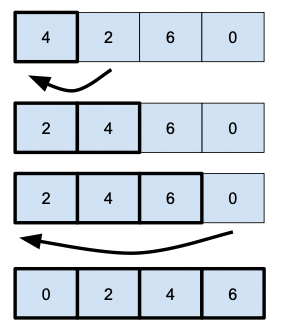
\includegraphics{images/insertion-sort.png}
\end{column}
\end{columns}
\end{frame}

\begin{frame}[fragile]{Live Coding:}
\protect\hypertarget{live-coding}{}
The \emph{h-index} is defined by Wikipedia as the maximum value of \(h\)
such that the given researcher has published at least \(h\) papers that
have each been cited at least \(h\) times.

Given a list of integers representing a researcher. Each index is their
\(ith\) publication and the value at the \(ith\) index is the number of
citation. Calculate the h-index of that researcher.

\begin{block}{Example}
\protect\hypertarget{example}{}
\begin{Shaded}
\begin{Highlighting}[]
\CommentTok{\# INPUT}
\NormalTok{lst }\OperatorTok{=}\NormalTok{ [}\DecValTok{2}\NormalTok{,}\DecValTok{2}\NormalTok{,}\DecValTok{5}\NormalTok{,}\DecValTok{6}\NormalTok{]}
\CommentTok{\# OUTPUT}
\DecValTok{2}
\end{Highlighting}
\end{Shaded}
\end{block}
\end{frame}

\hypertarget{hash-map-hash-table-python-dictionary-hash-functions}{%
\section{Hash map, hash table (Python dictionary), hash
functions}\label{hash-map-hash-table-python-dictionary-hash-functions}}

\begin{frame}{Motivating Example}
\protect\hypertarget{motivating-example-1}{}
\begin{itemize}
\item
  Recall from the first lecture that searching in a Python set took
  (basically) 0 seconds

  \begin{itemize}
  \item
    How was this achieved?
  \item
    Binary search only has \(O(\text{log}n)\) time, so there must be
    something else
  \end{itemize}
\item
  To achieve \(O(1)\) time, we need something that immediately knows the
  where/what the item is.

  \begin{itemize}
  \tightlist
  \item
    This is the purpose of \emph{hash functions}
  \end{itemize}
\end{itemize}
\end{frame}

\begin{frame}[fragile]{Hash Functions}
\protect\hypertarget{hash-functions}{}
\begin{itemize}
\item
  A hash function is a function where you enter a string and it returns
  an integer

  \begin{itemize}
  \tightlist
  \item
    Python objects have hash
  \end{itemize}
\end{itemize}

\begin{Shaded}
\begin{Highlighting}[]
\BuiltInTok{hash}\NormalTok{(}\StringTok{"DS 4 Life"}\NormalTok{)}
\end{Highlighting}
\end{Shaded}

\begin{verbatim}
-4234464436397453779
\end{verbatim}

\begin{itemize}
\item
  There are two requirements for a hash function

  \begin{itemize}
  \item
    It needs to be consistent. For instance, if you enter ``UofT'' and
    get ``1827'', then every time you enter ``UofT'' you should get
    ``1827''
  \item
    It maps different words to different numbers. Each string has a
    unique hash.
  \end{itemize}
\end{itemize}
\end{frame}

\begin{frame}{Using Hash Functions: Example}
\protect\hypertarget{using-hash-functions-example}{}
\begin{itemize}
\item
  Suppose you have a grocery store catalog with prices and barcodes.
  When you scan an item at checkout, you want it to instantly return the
  price.
\item
  You can put each barcode into a hash function.

  \begin{itemize}
  \item
    Let's say barcode ``1234'' \emph{hashes} to ``1'' and ``2'' hashes
    to ``9876''
  \item
    We store the price of item ``1234'' at address ``1''. Store the
    price of item ``4321'' at address ``2''
  \item
    We say the price at ``1'' is the \emph{hash value} of ``1''
  \end{itemize}
\item
  If there are 8 items sold at the store, then the hash function will
  only return integers from 1 to 8

  \begin{itemize}
  \item
    The size of the hash table is often referred to as its number of
    bins or slots.
  \item
    Thus, the hash function depends on the array
  \end{itemize}
\item
  This implementation is called a \emph{hash table}

  \begin{itemize}
  \tightlist
  \item
    The hash table is basically a list of lists, and the hash function
    maps an object to its location in the outer list.
  \end{itemize}
\end{itemize}
\end{frame}

\begin{frame}[fragile]{Python's Hash Tables: \texttt{dict}}
\protect\hypertarget{pythons-hash-tables-dict}{}
\begin{itemize}
\item
  You will likely never implement a hash table yourself, most languages
  have an implementation for has tables.

  \begin{itemize}
  \tightlist
  \item
    In Python, this is the \texttt{dict} class
  \end{itemize}
\item
  Dictionaries have keys and values (barcodes and prices)
\item
  Dictionaries have really good performance. Search, insert, or delete
  item are all are \(O(1)\) in the average case.

  \begin{itemize}
  \item
    Average case assumes you have a ``good'' hash function that avoids
    \emph{collisions}. You can read more about collisions in the
    textbooks.
  \item
    The worst case of Python dictionaries for search, insert, and delete
    is \(O(n)\).
  \end{itemize}
\item
  Recall Python dictionaries don't allow duplicate keys, that is because
  has hashes must be unique!
\end{itemize}
\end{frame}

\begin{frame}{Python \texttt{set}}
\protect\hypertarget{python-set}{}
\begin{itemize}
\item
  Recall during the first lecture, we showcased that Python's set search
  was much faster than list search
\item
  This is because Python's set implements a hash function to store its
  values
\end{itemize}
\end{frame}

\hypertarget{recommended-problems-and-references}{%
\section{Recommended Problems and
References}\label{recommended-problems-and-references}}

\begin{frame}[fragile]{Recommended Problems}
\protect\hypertarget{recommended-problems}{}
\begin{itemize}
\item
  Bhargava: Chapter 5

  \begin{itemize}
  \item
    5.1 to 5.4
  \item
    Read pages 79 to 86 on the use cases of hash functions
  \end{itemize}
\item
  Additional

  \begin{itemize}
  \item
    Give examples of 2 situations to use a queue and 2 situations to use
    a stack
  \item
    In Python, code a \texttt{stack} class with \texttt{is\_empty},
    \texttt{push}, and \texttt{pop} methods using the end of a Python
    list as the top of the stack. Bonus: Compare the run time of using
    the start of the list versus the end of the list as the top of the
    stack using the \texttt{timeit} library!
  \item
    In Python, code a \texttt{binary\_search} function.
  \item
    In Python, code a \texttt{hash\_table} that can hash 4 values.
  \end{itemize}
\end{itemize}
\end{frame}

\begin{frame}{References}
\protect\hypertarget{references}{}
\begin{itemize}
\item
  Bhargava, A. Y. (2016). \emph{Grokking algorithms: An illustrated
  guide for programmers and other curious people.} Manning. Chapter 5.
\item
  Cormen, T. H. (Ed.). (2009). \emph{Introduction to algorithms} (3rd
  ed). MIT Press. Chapter 2, 10, 11.
\item
  Horton, D., \& Liu, D. (2023, November 19). \emph{CSC148 Lecture
  Notes}.
  https://www.teach.cs.toronto.edu/\textasciitilde csc148h/winter/notes/
\end{itemize}
\end{frame}



\end{document}
